\documentclass[../szamtud.tex]{subfiles}

\begin{document}

    \subsection{Síkbarajzolhatóság}

        \textcolor{blue}{\textbf{Def:}} \textcolor{red}{Síkbarajzolt} (\textcolor{red}{SRt}) gráf alatt olyan gráfdiagramot értünk, amiven az  élek nem keresztezik egymást.

        A $G$ gráf \textcolor{red}{síkbarajzolható} (\textcolor{red}{SRható}), ha van SRt diagramja. 

        Síkbarajzolt gráf \textcolor{red}{tartománya} (\textcolor{red}{lapja}): a diagram komplementerének összefüggő tartománya. A nem korlátos rész neve \textcolor{red}{külső tartomány}. 

        \textcolor{blue}{\textbf{Megj:}} (1) A fentieket nem csak egyszerű gráfokra definiáltuk. (2) A SRt gráf nem csupán egy gráf, hanem egy \textbf{konkrét} diagram. (3) Ugyanannak a SRható gráfnak nagyon sok lényegesen különböző síkbarajzolt diagramja (lerajzolása) lehet. (4) A görbe (tóruszra) rajzolhatóság hasonlóan definiálható.

        \textcolor{orange}{\textbf{Állítás:}} (A $G$ gráf SRható) $\Longleftrightarrow$ ($G$ gömbre rajzolható) 

        \textcolor{green}{\textbf{Biz:}} A sztereografikus projekcióban az északi-sarkból történő vetítés kölcsönösen egyértelmű megfeleltetés a sík pontjai és a síkot a déli-sarkon érintő gömbfelszín pontjai (mínusz északi-sark) között. A síkbarajzolt diagram vetülete gömbre rajzolt lesz ($\Rightarrow$ \checkmark), és az \textit{É}-t nem tartalmazó gömbre rajzolt diagram pedig síkbarajzolttá válik. A $\Leftarrow$ irány igazolásához csupán annyi kell, hogy úgy rajzoljuk $G$-t a gömbre, hogy az \textit{É}-n ne menjen át él. \textcolor{blue}{$\Box$}

        \textcolor{orange}{\textbf{Köv:}} SRt gráf külső tartománynak nincs kitüntetett szerepe.

        \textcolor{green}{\textbf{Biz:}} Bármely lerajzolás "kifordítható": a diagram átrajzolható úgy, hogy a kiválasztott tartomány legyen a külső tartomány.

        \begin{enumerate}
            \item Vetítsük fel a diagramot a gömbre.
            \item Állítsuk az \textit{É}-t a kiválasztott tartománynak megfelelő gömbi tartomány belsejébe.
            \item Vetítsük vissza a gömbre rajzolt gráfot a síkra. \textcolor{blue}{$\Box$}
        \end{enumerate}

        \textcolor{orange}{\textbf{Köv:}} Bármely konvex poliéder élhálója SRható gráf.

        \textcolor{green}{\textbf{Biz:}} A $kx$ poliéder belső pontjából az élháló kivetíthető egy, a poliédert tartalmazó gömbre. Így az élhálóból göbmre rajzolt gráf lesz. Láttuk, hogy minden gömbre rajzolható gráf SRható. \textcolor{blue}{$\Box$}

        \textcolor{blue}{\textbf{Megj:}} A $kx$ poliéder élgráfjának tartományai a poliéder lapjainak felelnek meg.

        \textcolor{violet}{\textbf{Terminológia:}} SRt $G$ gráf esetén \textcolor{red}{$n, e, t$} ill. \textcolor{red}{$k$} jelöli rendre a $G$ csúcsai, élei, tartományai és komponensei számát.

        \textcolor{orange}{\textbf{Duális kézfogáslemma (DKFL):}} Ha $G$ SRt gráf, akkor $\sum_{i=1}^{t} l_i=2e$ ahol $l_i$ az $i$-dik lapot határoló élek számát jelöli.

        \textcolor{green}{\textbf{Biz:}} Minden él vagy két különböző lapot határol, vagy ugyanazt a lapot 2-szer. Így minden él 2-vel járul a BO-hoz és a JO-hoz is. \textcolor{blue}{$\Box$}

        \textcolor{blue}{\textbf{Megj:}} A DKFL akkor hasznos, ha a SRt gráf lapjairól, a KFL pedig akkor, ha a fokszámokról van információnk.

        \textcolor{orange}{\textbf{Fáry-Wagner-tétel:}} Ha $G$ egyerű SRható gráf, akkor olyan síkbarajzolása is van, amiben minden él egyenes szakasz.

    \subsection{Az Ezler-féle poliéderformula, síkgráfok karakterizációja}

        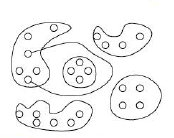
\includegraphics[width=0.2\textwidth]{./img/1.png}

        \textcolor{orange}{\textbf{Tétel:}} Ha $G$ SRt gráf, akkor $n+t=e+k+1$. 

        \textcolor{green}{\textbf{Biz:}} Rajzoljuk meg $G$-t az $n$ csúcsból kiindulva, az élek egyenkénti behúzásával. Kezdetben $t=1, e=0$ és $k=n$, így a bizonyítandó összefüggés fennáll. Tegyük fel, hogy már néhány élt berajzoltunk, még mindig fennáll az összefüggés, és egy éppen az $uv$ élt rajzolunk meg.

        $\boxed{1.}$ $u$ és $v$ különböző komponenshez tartoznak. Ekkor $k$ értéke 1-gyel csökken, $e$-é pedig 1-gyel nő. Az ÉHL miatt nem keletkezik kör, tehát nem zárunk körül új tartományt, vagyis $t$ nem változik. Az összefüggés fennmarad.

        $\boxed{2.}$ $u$ és $v$ ugyanahhoz a komponenshez tartoznak. Ekkor $k$ nem változik, $e$ viszont 1-gyel nő. Az ÉHL miatt keletkezik kör, tehát kettévágjuk az $uv$ élt tartalmazó korábbi tartományt. Ezért $t$ is 1-gyel nő, az összefüggés ismét fennmarad. \textcolor{blue}{$\Box$}

        \textcolor{orange}{\textbf{Köv:}} \textcolor{orange}{\textbf{(1)}} Ha $G$ SRható, akkor $t$ nem függ a síkbarajzolástól.

        \textcolor{green}{\textbf{Biz:}} $t = e + k + 1 - n$, és a JO nem függ a síkbarajzolástól. \textcolor{blue}{$\Box$}

        \textcolor{orange}{\textbf{(2)}} (\textbf{Euler-formula}) Ha $G$ összefüggő SRt gráf, akkor $n + t = e + 2$

        \textcolor{green}{\textbf{Biz:}} Mivel $G$ összefüggő, ezért a fenti Tételben $k = 1$. \textcolor{blue}{$\Box$}

        \textcolor{orange}{\textbf{(3)}} Ha $G$ egyszerű, SRható és $n \geq 3$, akkor $e \leq 3n - 6$.

        \textcolor{green}{\textbf{Biz:}} Ilyenkor $G$ minden lapját legalább 3 él határolja, így a DKFL miatt $2e = \sum_{i=1}^{t} l_i \geq 3t$. A Tétel alapján $3n + 2e \geq 3n + 3t = 3e + 3k \geq 3e + 3 + 3 = 3e + 6$, amit rendezve $e \leq 3n - 6$ adódik. \textcolor{blue}{$\Box$}

        \textcolor{orange}{\textbf{(4)}} $G$ egyszerű, SRható, $C_3$-mentes és $n \geq 3 \Rightarrow e \leq 2n - 4$. 

        \textcolor{green}{\textbf{Biz:}} Ilyenkor $G$ minden lapját legalább 4 él határolja. A DKFL miatt $2e = \sum_{i=1}^{t}l_i \geq 4t$, így $e \geq 2t$. A Tétel miatt $2n + e \geq 2n + 2t = 2e + 2k + 2 \geq 2e + 2 + 2 = 2e + 4$ Ezt rendezve $e \leq 2n - 4$ adódik. \textcolor{blue}{$\Box$}

        \textcolor{orange}{\textbf{(5)}} Ha $G$ egyszerű, SRható, akkor $\delta(G) \leq 5$ (azaz $\exists v : d(v) \leq 5$).

        \textcolor{green}{\textbf{Biz:}} A KFL és \textcolor{orange}{\textbf{(3)}} miatt $\sum_{v\in V(G)}d(v) = 2e \leq 6n - 12$. Ezért van olyan csúcs, amire $d(v) \leq \frac{6n-12}{n} < 6$. \textcolor{blue}{$\Box$}

        \textcolor{orange}{\textbf{(6)}} A $K_5$ és $K_{3,3}$ gráfok egyike sem SRható.

        \textcolor{green}{\textbf{Biz:}} A $K_5$ gráf egyszerű, de nem teljesül \textcolor{orange}{\textbf{(3)}}, hiszen $|E(K_5)| = \binom{5}{2} = 10 \nleq 9 = 3 \cdot 5 - 6$. Ezért $K_5$ nem SRható. A $K_{3,3}$ gráf egyszerű és $C_3$-mentes, de nem teljesül rá \textcolor{orange}{\textbf{(4)}}, u.i. $|E(K_{3,3})| = 9 \nleq 8 = 2 \cdot 6 - 4$. Ezrét $K_{3,3}$ nem SRható. \textcolor{blue}{$\Box$}

        \textcolor{blue}{\textbf{Megj:}} Könnyen látható, hogy ha $G$ SRható, akkor $G + e$ tóruszra rajzolható bármely $e$ él behúzása esetén. Nem nehéz látni, hogy $K_6$ is tóruszra rajzolható. Sőt: még $K_7$ is az, de $K_8$ már nem. 

        \textcolor{blue}{\textbf{Def:}} \textcolor{red}{Élfelosztás}: az élre egy új, másodfokú csúcs ültetése. \textcolor{red}{Élüsszehúzás}: az él törlése és két végpontjának azonosítása. \textcolor{red}{Topologikus G} (\textcolor{red}{soros bővítés}): $G$-ből élfelosztásokkal képzett gráf. 

        \textcolor{orange}{\textbf{Megf:}} Az éltörlés, csúcstörlés, élfelosztás, élösszehúzás operációk mindegyike megőrzi a gráf SRható tulajdonságát. 

        \textcolor{orange}{\textbf{Köv:}} (1) Top. $K_5$ top. $K_{3,3}$ nem SRható. (2) Ha $G$ SRható, akkor $G$-nek nincs se topologikus $K_5$, se topologikus $K_{3,3}$ részgráfja.

        \textcolor{orange}{\textbf{Kuratowski tétele:}} ($G$ SRható) $\Longleftrightarrow$ ($G$-nek nincs se topologikus $K_5$, se topologikus $K_{3,3}$ részgráfja) \textcolor{violet}{\textbf{Példa:}} Petersen-gráf

    \subsection{Síkgráfok duálisa}

        \textcolor{blue}{\textbf{Def:}} A $G$ SRt gráf \textcolor{red}{duálisa} a $G^*$ gráf, ha $G^*$ csúcsai $G$ tartományainak, $G^*$ élei $G$ éleinek felelnek meg. Az $uv \in E(G)$ élnek megfelelő duális él az $uv$ él által határolt két tartománynak megfelelő duális csúcsokat köti össze. 

        \textcolor{orange}{\textbf{Megf:}} (1) A SRt $G$ gráf $G^*$ duálisa SRható. ($n^*, e^*, t^*, k^*$) (2) $n^* = t, e^* = e, k^* = 1$. (3) Ha $v$ az $i$-dik laphoz tartozó duális csőcs, akkor $d_{G^*}(v) = l_i$.

        \textcolor{orange}{\textbf{Köv:}} KFL a duálisra $\sum_{i = 1}^{t} l_i = \sum_{v \in V(G^*)}d_{G^*}(v) = 2e^* = 2e$.

        \textcolor{blue}{\textbf{Def:}} A $Q \subseteq E(G)$ élhalmaz a $G$ gráf \textcolor{red}{vágása}, ha $G - Q$ szétesik (több komponense van, mint $G$-nek), de $Q' \subsetneq Q$ esetén $G - Q'$ nem esik szét. \textcolor{red}{Elvágó él:} egyélű vágás. \textcolor{red}{Soros élek}: kétélű vágás.

        \textcolor{orange}{\textbf{Kör-vágás dualitása:}} Tegyük fel, hogy $G^*$ a $G$ SRt gráf duálisa. Ekkor ($C$ a $G$ köre) $\Longleftrightarrow$ ($C^*$ a $G^*$ vágása) ill. ($Q$ a $G$ vágása) $\Longleftrightarrow$ ($Q^*$ a $G^*$ köre). 

        \textcolor{orange}{\textbf{Köv:}} Hurokél duálisa elvágó él, soros élpáré párhuzamos élpár.

    \subsection{Whitney} 

        \textcolor{orange}{\textbf{Whitney tétele:}} Tegyük fel, hogy $G^*$ a $G$ SRt gráf duálisa. Ekkor $H$ pontosan akkor duálisa a $G$ egy alkalmas síkbarajzolásának, ha $H$ előáll $G^*$-ból a fenti Whitney-operációk alkalmas egymásutánjával.

        \textcolor{blue}{\textbf{Def:}} A $\varphi : E(G) \rightarrow E(H)$ kölcsönös egyenértékű leképezés \textcolor{red}{kör-vágás dualitás} $G$ és $H$ között, ha $C$ pontosan akkor $G$ köre, ha $\varphi(C) H$ vágása.

        \textcolor{orange}{\textbf{Whitney másik tétele:}} Tegyük fel, hogy $G$ és $H$ között kör-vágás dualitás van. Ekkor $G$ SRható, és $H$ a $G$ egy alkalmas síkbarajzolásának duálisa.
        
        \textcolor{blue}{\textbf{Megj:}} Egy $G$ gráf által leírt villamos hálózat viselkedését az Ohm-él Kirchhoff-törvények írják le. Ezek a $G$ gráf éleire, köreire és vágásaira vonatkoznak. Ha $G$ és $H$ közt kör-vágás dualitás van, akkor $H$-n elkészíthető az előző hálózat duálisa. Az eredeti hálózat megoldásában ha az I és U értékeket felcsréljük, az utóbbi hálózat megoldását kapjuk. Whitney másik tétele miatt ez a különös szimmetria csak SRható gráfok által leírt hálózatokon lehetséges.

\end{document}